% =============================================================================
% Chapter 5 — The Fabric: RoCE, NCCL, and the Art of Not Pinning
% =============================================================================
\chapter{The Fabric: RoCE, NCCL, and the Art of Not Pinning}
\label{ch:fabric}

Each DGX Spark in this deployment advertises a 200\,Gb/s QSFP port --- and no
single PCIe function behind that port can carry it. Why that is true, how an
audit proved it, and what it demands of every layer above it is where this
chapter begins (\Cref{sec:fabric-physical}).

The stakes are concrete: every decode step moves roughly 108 NCCL
collectives across the direct QSFP cable between the two machines. Every
prefill chunk pushes hundreds of megabytes of all-reduce traffic over the
same link that also carries the worker's model weights at boot. This chapter
is the fabric layer of the handbook --- how one ConnectX-7 ASIC turns into
four PCIe functions, how NCCL actually parses the device selector you hand
it, why this repository stopped pinning RoCEv2 GID indexes and started validating
them instead, and what evidence a frozen tensor-parallel pair leaves behind
when the forensics were wired in advance. The habits transfer to any
multi-node serving stack, whatever the NIC vendor: verify the PCIe topology
before tuning the network, validate rather than pin, treat defined-empty
environment variables as a distinct hazard, instrument before the incident.

\section{The physical layer: one ASIC, four functions}
\label{sec:fabric-physical}

Each DGX Spark exposes its 200\,Gb/s QSFP networking through a single
ConnectX-7 (CX7) ASIC. The surprise, confirmed during the fable5-1 audit of
2026-09-02 by matching \code{sys_image_guid} across devices, is that this one
ASIC presents \emph{four} PCIe functions to the host: two physical ports, and
\emph{two PCIe functions per port} --- a socket-direct layout. Each physical
function (PF) is wired PCIe Gen5 $\times$4, which is about 15.7\,GB/s
$\approx$ 126\,Gb/s of raw PCIe bandwidth (the launcher's comments call it
``$\sim$100G each'' in practice). The arithmetic is unforgiving: a single PF
cannot carry the port's 200\,Gb/s. Reaching full port rate requires NCCL to
drive \emph{both} PFs of the port at once --- which is exactly what the
dual-HCA configuration in \Cref{sec:fabric-measured} does.

\begin{figure}[htbp]
\centering
\begin{tikzpicture}[font=\small]
  % ---- Spark 1 (head) ----
  \node[hbgpu,minimum width=32mm] (gpu0) {GB10 GPU\\rank 0 (head)};
  \node[hbnode,below=10mm of gpu0.south west,anchor=north west,
        font=\scriptsize] (pf00) {PF f0\\Gen5 $\times$4};
  \node[hbnode,right=3mm of pf00,font=\scriptsize] (pf01) {PF f1\\Gen5 $\times$4};
  \begin{scope}[on background layer]
    \node[hbgroup,fit=(pf00)(pf01),
          label={[hblabel]below:{CX7 ASIC, one QSFP port}}] (cx0) {};
  \end{scope}
  \draw[hbarrow,<->] (gpu0.south) -- (cx0.north);
  % ---- Spark 2 (worker) ----
  \node[hbgpu,minimum width=32mm,right=62mm of gpu0] (gpu1)
        {GB10 GPU\\rank 1 (worker)};
  \node[hbnode,below=10mm of gpu1.south west,anchor=north west,
        font=\scriptsize] (pf10) {PF f0\\Gen5 $\times$4};
  \node[hbnode,right=3mm of pf10,font=\scriptsize] (pf11) {PF f1\\Gen5 $\times$4};
  \begin{scope}[on background layer]
    \node[hbgroup,fit=(pf10)(pf11),
          label={[hblabel]below:{CX7 ASIC, one QSFP port}}] (cx1) {};
  \end{scope}
  \draw[hbarrow,<->] (gpu1.south) -- (cx1.north);
  % ---- RoCE link ----
  \draw[hbflow,<->,very thick] (cx0.east) -- (cx1.west)
    node[midway,above=1mm,align=center,font=\scriptsize,fill=white,
         inner sep=1.5pt]
    {direct QSFP, 200 Gb/s RoCEv2\\NCCL collectives (RDMA)\\
     Gloo/TCPStore bootstrap, ZMQ scheduler (TCP)\\NFS weight reads (TCP)};
  % ---- LAN ----
  \node[hbfaint,below=31mm of gpu0,minimum width=30mm,font=\scriptsize]
        (lan0) {mgmt LAN port};
  \node[hbfaint,below=31mm of gpu1,minimum width=30mm,font=\scriptsize]
        (lan1) {mgmt LAN port};
  \draw[hbarrow,dashed,<->] (lan0.east) -- (lan1.west)
    node[midway,below=6mm,align=center,font=\scriptsize,fill=white,
         inner xsep=4pt,inner ysep=1.5pt]
    {management LAN: SSH orchestration, client API traffic};
  \draw[hbarrow,dashed] (gpu0.west) to[out=180,in=180] (lan0.west);
  \draw[hbarrow,dashed] (gpu1.east) to[out=0,in=0] (lan1.east);
\end{tikzpicture}
\caption{Two-node topology. Each Spark's 200\,Gb/s QSFP port is backed by one
CX7 ASIC exposing two PCIe functions, each Gen5 $\times$4
($\approx$126\,Gb/s), so full port rate needs both PFs. NCCL RDMA, the
Gloo/TCPStore bootstrap, the per-step ZMQ scheduler broadcast, and optional
NFS weight loading all ride the CX7 link (via its IP interfaces); the
launcher's SSH control plane and client API traffic use the management LAN.}
\label{fig:fabric-topology}
\end{figure}

The fable5-1 audit (finding 3, priority P1) inspected both hosts read-only and
found the fabric healthy at the RDMA layer but mistuned at almost every layer
beneath it. \Cref{tab:fabric-health} summarizes the evidence.

\begin{table}[htbp]
\centering\small
\caption{Fabric health snapshot from the fable5-1 audit (2026-09-02, both
nodes, read-only inspection).}
\label{tab:fabric-health}
\begin{tabular}{l>{\raggedright\arraybackslash}p{5.0cm}>{\raggedright\arraybackslash}p{5.2cm}}
\toprule
Observable & Measured & Implication \\
\midrule
RoCE \code{active_mtu} & 1024 (max 4096) & Ethernet MTU 1500 caps IB MTU \\
Ethernet MTU & 1500 (max 9978) & RoCE 4096 needs Ethernet $\geq$ 4200 \\
NIC rings & 1024 (max 8192) & buffer-limited bursts \\
RoCE hw retransmits & 0 & link itself is clean \\
Pause frames & both directions; 1.7\,s tx (head) & global pauses stall NCCL too \\
\code{rx_out_of_buffer} & 13{,}071 (worker) & bursts overflow 1024-slot rings \\
FEC-corrected lane errors & tens of millions & absorbed by RS-FEC; check cable \\
Second-PF subnet & duplicate 10.0.22.0/24 & ARP flux; RTT 0.70 vs.\ 0.33\,ms \\
\bottomrule
\end{tabular}
\end{table}

Three of these deserve unpacking for a reader who has not wired RoCE before.
First, RoCE derives its InfiniBand-side MTU from the Ethernet netdev MTU: with
the stock Ethernet 1500, the RoCE \code{active_mtu} settles at 1024 bytes, and
every RDMA message fragments accordingly. Getting RoCE to its 4096 maximum
requires Ethernet at 4200 or more --- which is why the tuning work in
\Cref{sec:fabric-measured} jumps straight to 9000.

Second, the pause frames
observed here are \emph{global} Ethernet pauses, not priority flow control ---
when the receiver's 1024-entry rings overflow during a burst (the audit
suspected the NFS weight load sharing the link), the pause stalls
\emph{everything} on the wire, NCCL included.

Third, the second PF on each
node carried addresses \code{10.0.22.101}/\code{.102} on the same wire as
\code{10.0.22.1}/\code{.2}. Linux answers ARP for any local address on any
interface, so a duplicate subnet on two interfaces produces textbook ARP flux,
visible as the doubled RTT through the second PF. The audit flagged
de-duplicating that subnet before trusting any dual-PF configuration.

The consequences are asymmetric. Decode collectives are small
($\sim$344\,KB at concurrency 6) and latency-bound, so link bandwidth barely
touches them. Prefill is another story: each 1024-token chunk performs 86
all-reduces of $\sim$8\,MB ($\approx$690\,MB per chunk per rank) plus a
10.9\,MB logits all-gather. At $\sim$11\,GB/s on a single PF that is
$\sim$60\,ms per chunk --- around 15\,\% of a short-context chunk's step time.
This is why the fabric findings promise ``prefill comm bandwidth up to
$\sim$2$\times$; decode $\approx$ unchanged.'' Claiming that 2$\times$,
though, first requires naming the right devices to NCCL --- which is where
the launcher's troubles begin.

\section{Device selection: the NCCL\_IB\_HCA grammar}
\label{sec:fabric-selector}

The launcher must answer a question NCCL never has to: \emph{before}
starting either container, do all the devices this selector will pick
actually have usable RoCEv2 addressing? Answering it requires knowing
exactly what the selector means --- and \envvar{NCCL_IB_HCA} looks like a
device name but is actually a small language. NCCL's \code{parseStringList}
(in \code{src/misc/utils.cc}) accepts an optional leading \code{^} meaning
\emph{exclude the matches}, then an optional \code{=} meaning \emph{exact
name match} instead of the default prefix match, then a comma-separated list
of \code{name[:port[:rail[:plane]]]} tokens. The fine print matters
operationally:

\begin{itemize}
  \item Empty names are dropped, only the first 32 non-empty entries
        (\code{MAX_IB_DEVS}) are stored --- later entries are silently
        ignored --- and each stored name is truncated to the 63-byte payload
        of \code{netIf::prefix} before matching.
  \item An absent \emph{or empty} port field means $-1$, ``any port'':
        \code{devA} and \code{devA:} select exactly the same thing.
  \item A non-empty port field goes through \code{atoi()} --- optional
        whitespace and sign, then leading decimal digits, stopping at the
        first non-digit --- so \code{:08} is decimal port 8 (never octal),
        and \code{:abc} is port 0, which matches no real port.
\end{itemize}

Rail and plane fields are parsed off and ignored for matching here.

Just as important is \emph{what the selector is applied to}. NCCL's
\code{ncclIbInit} builds a candidate universe first: only ports that are
\code{ACTIVE} and whose link layer is Ethernet or InfiniBand, capped again at
32 entries --- and both filters run \emph{before} \envvar{NCCL_IB_HCA} is
consulted. A \code{DOWN} sibling port, common on these dual-port cards, is
simply never a candidate: it cannot fail a match, and NCCL never opens it. A
plain prefix selector like \code{roce} therefore works even on a node where
half the ports are unused. Selection is therefore two filters in series ---
the universe NCCL builds, then the selector the operator writes --- and a
tool that models only the second one will happily validate devices NCCL was
never going to open (\Cref{fig:fabric-hca-selector}).

\subsection{Why the launcher mirrors the grammar byte-for-byte}

To answer the question that opened this section, the start script carries a
shell reimplementation of the selector grammar --- the
\envvar{NCCL_HCA_RESOLVER_BODY} heredoc in
\repofile{start-deepseek-v4-flash-dspark.sh}. The script ships it over SSH
to run \emph{on the node that owns the sysfs tree}, because
\repofile{/sys/class/infiniband} is only meaningful locally. The body is a
quoted heredoc (nothing expands at definition time), and
\code{resolve_rocev2_gid_index} prepends the inputs as \texttt{printf \%q}
assignments so selector tokens travel literally. The resolver runs under
\code{set -f} so a token like \code{roce*} can never glob-expand against the
remote filesystem.

The original version of this resolver, fixed in the 2026-08-20 changelog
entry, used the raw \envvar{NCCL_IB_HCA} value as a sysfs directory name.
Any selector syntax at all --- including the recommended deterministic exact
list \code{=devA,devB} --- produced a path like
\repofile{/sys/class/infiniband/=devA,devB/ports/1/gids} that matched
nothing, and the launcher exited before starting either rank. The rewrite
mirrors NCCL's semantics exactly: \code{^} exclusion, \code{=} exact
matching, the 32-entry cap, the 63-byte name truncation (via a
byte-oriented \texttt{LC\_ALL=C printf '\%.63s'}), and one \code{atoi}-style
conversion per port field.

The subtlest bug in that mirroring is worth a war story.

\begin{hbwarstory}
NCCL's \code{atoi()} happily reads a port number of any width; shell
arithmetic does not. Evaluating an arbitrary-width digit string with
\texttt{\$(( ))} wraps modulo $2^{64}$ --- and one specific input,
\num{18446744073709551615}, wraps to exactly $-1$. In this resolver $-1$ is
not an error value: it is the ``any port'' wildcard. An unrepresentably huge
port field would therefore have silently \emph{widened} the selection to
every port of the device instead of matching nothing. The fix refuses to
evaluate anything wider than a conservative nine digits and clamps it to a
port number no sysfs tree can contain, so the token matches nothing and the
resolve fails closed.
\end{hbwarstory}

The guard in the resolver:

\begin{lstlisting}[language=bash]
if [ -z "$mag" ]; then
  port=0
elif [ ${#mag} -gt 9 ]; then
  # Outside the conservative nine-digit bound. Evaluating arbitrary-width
  # text with $(( )) can wrap the value modulo 2^64 - and
  # 18446744073709551615 wraps to exactly -1, which is the "any port"
  # wildcard - so an unrepresentable port would silently *widen* the
  # selection. Clamp to a value no sysfs port can have: the token then
  # matches nothing and the resolve fails closed.
  port=${sign}999999999
else
  port=$(( 10#$mag ))
  [ -z "$sign" ] || port=$(( 0 - port ))
fi
\end{lstlisting}

The resolver also reproduces the candidate-universe rules: it walks
\repofile{/sys/class/infiniband}, keeps only \code{ACTIVE} ports with an
Ethernet or InfiniBand link layer, treats an \emph{unreadable} attribute as
``still a candidate'' (absence of evidence is not evidence of a down port),
applies the selector, and caps the result at 32, noting on stderr anything
NCCL would ignore. The whole construction is gated by
\repofile{scripts/test-nccl-ib-hca-gid-resolve.sh}, a 72-check suite that
runs the launcher's own generated script against fake sysfs trees ---
covering the 32/33 entry boundary, 63-byte truncation, the leading-zero and
overflow port forms, exclusions, prefix collisions, and DOWN-port handling
--- and fails behaviorally on the pre-fix launcher.

\begin{figure}[htbp]
\centering
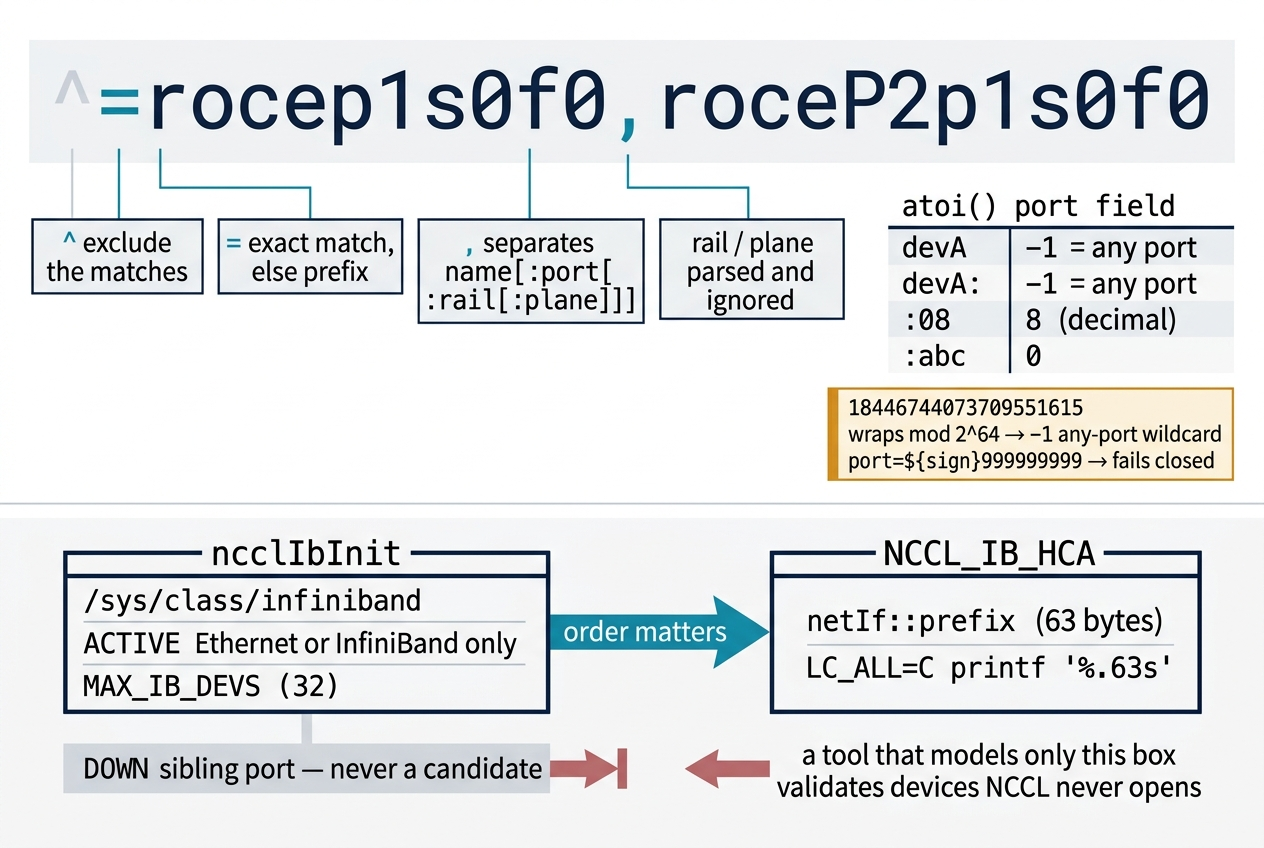
\includegraphics[width=\textwidth]{figures/ch05-hca-selector.png}
\caption{The \envvar{NCCL_IB_HCA} selector is a grammar applied to a universe
NCCL has already built. Top: token anatomy --- optional \code{^} exclusion,
optional \code{=} exact match, comma-separated
\code{name[:port[:rail[:plane]]]} --- with \code{atoi} port semantics, where
\code{devA} and \code{devA:} are both the $-1$ any-port wildcard, \code{:08}
is decimal 8 and \code{:abc} is port 0, and the nine-digit clamp that stops
\num{18446744073709551615} from wrapping to the wildcard. Bottom: selection
is two filters in series. \code{ncclIbInit} keeps only \code{ACTIVE}
Ethernet or InfiniBand ports, capped at 32, before the selector is consulted,
so a \code{DOWN} sibling port can never fail a match --- and a validator that
models only the selector checks devices NCCL was never going to open.}
\label{fig:fabric-hca-selector}
\end{figure}

\section{GID resolution: validate and leave unset}
\label{sec:fabric-gid}

The selector settles \emph{which} ports NCCL drives; addressing settles
whether it can reach anything through them. RoCEv2 identifies an endpoint by
a GID --- for IPv4-based RoCEv2, an
IPv4-mapped address ending in \code{ffff:aabb:ccdd} for \code{a.b.c.d} ---
and each HCA port exposes a small table of them, indexed by integer.
\envvar{NCCL_IB_GID_INDEX} tells NCCL which table entry to use. The trap is
that the usable index is a property of one port on one node at one moment:
it differs per HCA, differs per node, and drifts after reboots, firmware
updates, and link events, because the kernel rebuilds the GID table.

The repository's first answer (PR \ghissue{95} lineage) was to resolve a common
index across all selected members at launch and pin it. The 2026-08-20
resolver even reconciled members by \emph{intersecting} their usable index
sets, exiting with a distinct code when the intersection was empty --- since
\envvar{NCCL_IB_GID_INDEX} is one global value per rank, no single pin can
serve members that disagree. The 2026-09-02 change (credited to tonyd2wild
in issue \ghissue{38}) abandoned pinning entirely, and the reasoning is a
transferable lesson:

\begin{hblesson}
A pin is one global value per rank; the property it pins varies per HCA and
over time. Any pinned index --- including a correctly resolved intersection
--- can later wedge NCCL initialization (\code{ibv_modify_qp} error 61) on a
dual-HCA node after a link event moves the tables. When the underlying
system (NCCL selects the RoCEv2/IPv4 GID \emph{per HCA} whenever the
variable is absent) already does the right thing dynamically, the robust
launcher role is \emph{validation}, not \emph{configuration}: prove at start
time that every selected member has at least one usable GID, print the
evidence, and then leave the variable unset.
\end{hblesson}

Under the default \envvar{NCCL_IB_GID_AUTO}\code{=1}, the resolver therefore
runs in audit mode: for every selected HCA/port it collects \emph{all}
indexes whose GID type is \code{RoCE v2} and whose address matches either
the preferred match IP or an IPv4 on the member's own netdev. (One shared
match IP must not silently disqualify a member living on a different link
address.) Members with disjoint usable sets are fine --- nothing is being
reconciled.

A member with \emph{no} usable RoCEv2 GID is another matter: it aborts the
launch with per-member diagnostics (exit 1, fail closed), before any remote
side effect.

Match IPs come from \code{pick_gid_match_ip}, which prefers an explicit
\envvar{NCCL_IB_GID_MATCH_IP}, then the first IPv4 on the socket interface,
then the configured fabric IP, then the bare worker host address. Stale
\envvar{NCCL_IB_GID_INDEX} pins left in \repofile{.env.dspark} are reported
and ignored, and \envvar{NCCL_IB_GID_AUTO}\code{=0} restores verbatim
pinning for stacks where auto validation is unavailable.

\begin{figure}[htbp]
\centering
\begin{tikzpicture}[font=\small,node distance=5mm]
  \node[hbbox,text width=56mm] (sel) {NCCL\_IB\_HCA selector\\
    \texttt{[\^{}][=]name[:port],...}};
  \node[hbnode,below=of sel,text width=56mm] (parse)
    {Parse (mirrors \texttt{parseStringList}):\\
     32-entry cap, 63-byte names,\\ atoi ports, $2^{64}$-wrap clamp};
  \node[hbnode,below=of parse,text width=56mm] (univ)
    {Candidate universe from sysfs:\\ ACTIVE + Ethernet/InfiniBand\\
     link layer, cap 32 (as \texttt{ncclIbInit})};
  \node[hbnode,below=of univ,text width=56mm] (members)
    {Selected members (per node,\\ run over SSH on the sysfs owner)};
  \node[hbnode,below=of members,text width=56mm] (check)
    {Per member: any RoCE v2 GID\\ matching match-IP or an IPv4\\
     on the member's own netdev?};
  \node[hbwarn,below left=6mm and -22mm of check,text width=30mm]
    (fail) {FATAL, exit 1\\ (fail closed, per-member\\ diagnostics)};
  \node[hbgpu,below right=6mm and -22mm of check,text width=34mm]
    (ok) {Audit usable indexes\\ to stderr; leave\\
    NCCL\_IB\_GID\_INDEX\\ \emph{unset} on both ranks};
  \node[hbfaint,right=10mm of members,text width=26mm,font=\scriptsize]
    (pin) {AUTO=0:\\ pin env values\\ verbatim instead};
  \draw[hbflow] (sel) -- (parse);
  \draw[hbflow] (parse) -- (univ);
  \draw[hbflow] (univ) -- (members);
  \draw[hbflow] (members) -- (check);
  \draw[hbfail] (check.south) -- (fail.north)
    node[hblabel,midway,left=1mm] {none};
  \draw[hbok] (check.south) -- (ok.north)
    node[hblabel,midway,right=1mm] {$\geq 1$};
  \draw[hbarrow,dashed] (pin.west) -- (members.east);
\end{tikzpicture}
\caption{GID auto-resolution under \envvar{NCCL_IB_GID_AUTO}\code{=1}:
selector parse, NCCL-faithful candidate universe, per-member usable-GID
validation, then fail-closed abort or validate-and-leave-unset. NCCL itself
picks the RoCEv2/IPv4 GID per HCA when the index variable is absent.}
\label{fig:fabric-gid-flow}
\end{figure}

\begin{hbwarning}
For NCCL, \emph{empty is not absent}. A defined-but-empty
\envvar{NCCL_IB_GID_INDEX} parses as GID index 0, and because NCCL loads
\repofile{/etc/nccl.conf} (and \envvar{NCCL_CONF_FILE}) with
\code{overwrite=0}, a defined-empty environment variable also \emph{masks}
any config-file value. Compose makes this hazard structural: the compose
file necessarily defines the key. The stack defuses it in two places. The
launcher deliberately keeps emitting \envvar{NCCL_IB_GID_INDEX} --- empty
--- into the worker's SSH environment, so the empty process-level value
out-substitutes a stale pin in the worker's own \repofile{.env.dspark}. The
shared container entrypoint then \emph{unsets} every defined-empty
variable before \code{exec}, so what reaches NCCL is truly absent. Recreate
both ranks (stop then start) after switching modes, or the old in-container
pin survives in the writable layer.
\end{hbwarning}

\begin{figure}[htbp]
\centering
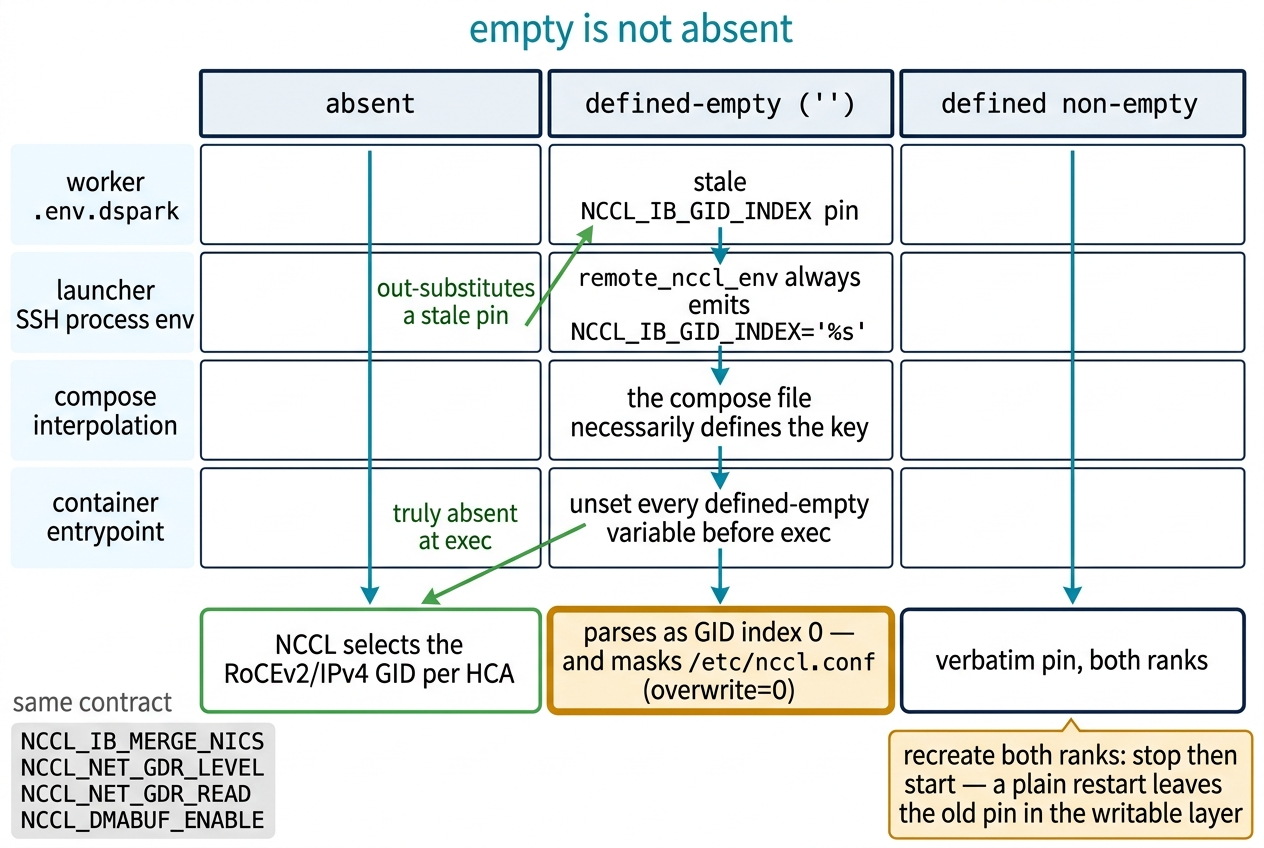
\includegraphics[width=\textwidth]{figures/ch05-empty-not-absent.png}
\caption{Absent, defined-empty, and defined are three different states to
NCCL. A defined-but-empty \envvar{NCCL_IB_GID_INDEX} parses as GID index 0
and, because NCCL loads \repofile{/etc/nccl.conf} with \code{overwrite=0},
also masks the config file --- a hazard Compose makes structural by always
defining the key. The stack defuses it twice: the launcher deliberately emits
the empty value so it out-substitutes a stale pin in the worker's own
\repofile{.env.dspark}, and the shared entrypoint unsets every defined-empty
variable before \code{exec}, so what reaches NCCL is truly absent. The same
contract governs the four fabric passthrough knobs.}
\label{fig:fabric-empty-not-absent}
\end{figure}

\section{Head/worker asymmetry: injecting the worker's view}
\label{sec:fabric-worker}

The warning above leaned on machinery this section owes an explanation: the
launcher deliberately injecting environment into the \emph{worker's} SSH
sessions. The reason is an asymmetry of naming. On a QSFP ring the worker's
port facing the head is often a
differently-named device than the head's port facing the worker, so one
shared \repofile{.env.dspark} cannot describe both nodes. Any mechanism that
feeds both ranks the same values points the worker's NCCL, Gloo, and
scheduler sockets at devices named for the head --- a misconfiguration made
at boot, before any collective can reveal it. The general form is worth
naming, because it recurs wherever a cluster is not symmetric: a setting
whose correct value differs per node cannot live in a file that every node
reads (\Cref{fig:fabric-worker-env}).

The repository's contract: set \envvar{WORKER_NCCL_IB_HCA},
\envvar{WORKER_NCCL_SOCKET_IFNAME}, \envvar{WORKER_TP_SOCKET_IFNAME}, and
\envvar{WORKER_GLOO_SOCKET_IFNAME} in the \emph{head's} env file, and the
launcher injects them into every remote \code{docker compose} invocation as
process environment over SSH. Docker Compose variable substitution is
explicitly ruled out for this job --- a \code{WORKER_*}-first default in the
compose file is not rank-aware, and a shared or scp'd env file would feed
both ranks the same values. Each worker variable defaults to its head
counterpart when unset, so single-name setups need nothing extra. The
injection point is \code{remote_nccl_env}:

\begin{lstlisting}[language=bash]
remote_nccl_env() {
  # Rebuild each call so GID resolve after early init is visible on the
  # worker. NCCL_IB_GID_INDEX is always emitted, even empty under
  # NCCL_IB_GID_AUTO=1: the empty process-env value overrides a stale
  # worker .env.dspark entry at compose interpolation, and the shared
  # entrypoint normalization makes the defined-empty variable truly
  # absent in the container (NCCL would parse a defined-empty value as
  # GID index 0).
  printf "NCCL_IB_HCA='%s' NCCL_SOCKET_IFNAME='%s' TP_SOCKET_IFNAME='%s' \
    GLOO_SOCKET_IFNAME='%s' NCCL_IB_GID_INDEX='%s' ..." \
    "$WORKER_NCCL_IB_HCA" "$WORKER_NCCL_SOCKET_IFNAME" \
    "$WORKER_TP_SOCKET_IFNAME" "$WORKER_GLOO_SOCKET_IFNAME" \
    "$WORKER_NCCL_IB_GID_INDEX"
}
\end{lstlisting}

Two properties of this function are load-bearing. It is rebuilt on every
call, so a GID resolution that happens after early initialization is still
visible to later remote compose commands. And it always emits
\envvar{NCCL_IB_GID_INDEX}, even empty, for exactly the masking reason
described in the hazard box above. The same pattern extends to a third node:
\code{remote_nccl_env2} emits the \envvar{WORKER2_NCCL_*} family for the
optional TP=3 lane (\Cref{ch:scaling}).

\begin{figure}[htbp]
\centering
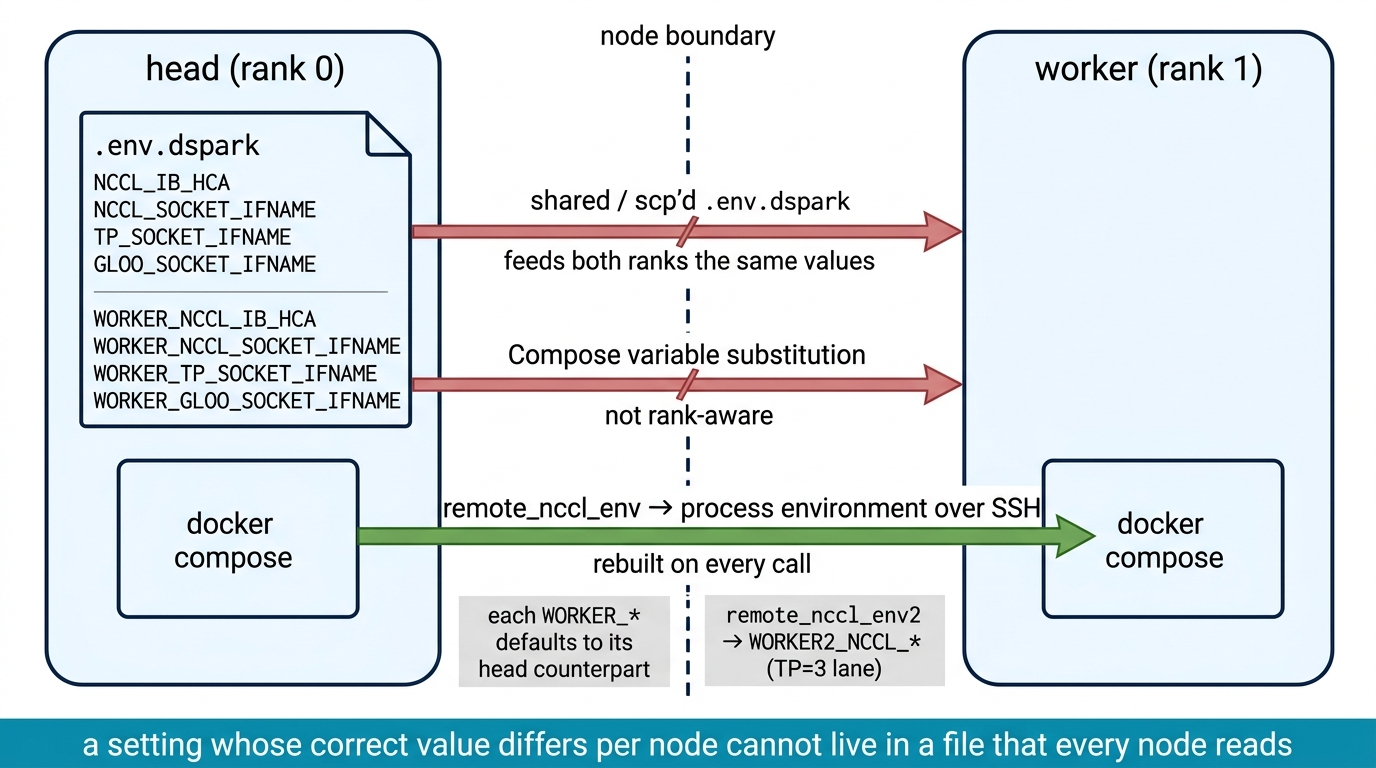
\includegraphics[width=\textwidth]{figures/ch05-worker-env-ssh.png}
\caption{Head/worker asymmetry. The worker's port facing the head is often a
differently named device than the head's port facing the worker, so one
shared \repofile{.env.dspark} cannot describe both nodes. Two plausible
mechanisms are ruled out --- a shared or \code{scp}'d env file and Compose
variable substitution both feed the worker values named for the head --- and
the launcher instead injects the \code{WORKER_*} family as process
environment into every remote \code{docker compose} call, rebuilding it per
call so a GID resolve after early init is still visible. Each
\code{WORKER_*} defaults to its head counterpart, and
\code{remote_nccl_env2} extends the pattern to the optional TP=3 lane.}
\label{fig:fabric-worker-env}
\end{figure}

\section{Measured fabric tuning: dual HCA and MTU 9000}
\label{sec:fabric-measured}

With both ranks guaranteed to address their own devices, the socket-direct
implication of \Cref{sec:fabric-physical} could finally be put to the test.
It was confirmed by measurement on 2026-08-21, on two independent
2$\times$\,GB10 TP=2 pairs with a direct QSFP cable. With only one PF in \envvar{NCCL_IB_HCA}, the link
runs at half the port. The measured configuration listed both controllers
with the deterministic exact-selector form (NIC merging is NCCL's default
behavior) and set MTU 9000 on both controller interfaces at both endpoints:

\begin{lstlisting}[language=bash]
NCCL_IB_HCA==rocep1s0f0,roceP2p1s0f0   # map names: ibdev2netdev
\end{lstlisting}

The results, exactly as the repository records them: pair 1 measured 1311 \tokspersec{}
at MTU 1500 with one HCA, 1343 \tokspersec{} at MTU 9000 with one HCA, and 1410
\tokspersec{} with both HCAs --- \textbf{+7.6\,\%} end-to-end from its own
baseline. Pair 2 reproduced a 1422 \tokspersec{} dual-HCA final rate but has no
same-pair single-HCA baseline, so the repository explicitly declines to quote an
uplift percentage for it --- a small but characteristic act of measurement
hygiene.

Two prerequisites were recorded alongside the numbers. Both interfaces must
be UP with IPs in \emph{distinct} subnets: the duplicate subnet of
\Cref{sec:fabric-physical} had doubled the second PF's round-trip time,
0.70 versus 0.33\,ms, so de-duplicating it is what makes the second PF
worth driving at all. And per-controller PCIe width must be verified
$\times$4 in sysfs (\code{current_link_width}) --- early BIOS revisions wire
the second controller $\times$2. On switched paths, jumbo frames are only safe when
every endpoint and intervening L2 hop is verified at the same MTU.

\begin{hbnote}
Do not transfer microbenchmark deltas to serving throughput. The same
dual-HCA change moved \code{nccl-tests} bus bandwidth by +64\,\% while
end-to-end throughput moved +7.6\,\%: the all-reduce is only a slice of
prefill step time. Engine-counter probes on the measured stack found no
material decode change (code 76.0 \tokspersec{} at 73.3\,\% draft acceptance,
prose 37.3 at 25.7\,\%, 14--15 steps/s) and an unchanged KV pool ---
consistent with decode collectives being latency-bound. The contrast case
is instructive too: an earlier \emph{unmerged} dual-HCA attempt
(2026-08-06), which split channels across two logical NICs instead of
merging both PFs into one, cost KV buffer memory for a +3\,\% result.
\end{hbnote}

Two more findings shape what the defaults do \emph{not} contain. First, no
GPUDirect RDMA was observed on the measured stack: on GB10 driver 580.173.02
the container reported \code{CU_DEVICE_ATTRIBUTE_DMA_BUF_SUPPORTED=0} and
boot logs showed host-staged transport (\code{via NET/IB/x}, no
\code{/GDRDMA}). Every collective therefore bounces through a host buffer,
which on unified memory is an extra GPU-side memcpy rather than a PCIe hop.
The repository is careful to scope this as a contributor-reported observation on
that stack only, not a claim about GDR in general.

Second, the four NCCL passthrough
knobs (\Cref{tab:fabric-passthrough}) all default to \emph{unset}, with a
precise absence contract. Compose necessarily defines each key, but the
entrypoint unsets empty definitions before \code{exec}, so NCCL's built-in
defaults and config-file values still apply and cannot be masked by a
defined-empty value. Configured non-empty values pass through unchanged on
both ranks (\Cref{fig:fabric-empty-not-absent}).

\begin{table}[htbp]
\centering\small
\caption{NCCL fabric passthrough knobs (all default unset; empty is
normalized to absent by the entrypoint).}
\label{tab:fabric-passthrough}
\begin{tabular}{lp{86mm}}
\toprule
Variable & Role \\
\midrule
\envvar{NCCL_IB_MERGE_NICS} & NCCL default is 1: \emph{permits} merging
compatible dual-port NICs into one logical device; it selects nothing and
forces nothing. The meaningful override is 0, to disable merging. \\
\envvar{NCCL_NET_GDR_LEVEL} & Upstream GPUDirect override; no effect
demonstrated on the submitted GB10 stack. \\
\envvar{NCCL_NET_GDR_READ} & Upstream GPUDirect override; same status. \\
\envvar{NCCL_DMABUF_ENABLE} & 0 disables DMA-BUF probing --- the meaningful
workaround control where probing misbehaves. \\
\bottomrule
\end{tabular}
\end{table}

Taken together, the tuning surface here is narrower than it looks. Two PFs
and MTU 9000 are the measured win; everything else in
\Cref{tab:fabric-passthrough} ships unset because nothing on this stack
demonstrated a reason to set it.

\section{Forensics: the flight recorder and the FIFO poke}
\label{sec:fabric-forensics}

A tuned and validated fabric can still freeze mid-collective --- and when it
does, what matters is the evidence it leaves behind. The mechanism below has
two halves, and both must be in place long before they are needed: a
recorder that runs on every boot, and a trigger an external watchdog can
pull on a rank that is frozen but has not yet timed out. Every tensor-parallel
pair loss in this deployment's history (the issue
\ghissue{117} class, and the stochastic \ghissue{141} stalls of
\Cref{ch:bugs}) ended the same way: the stalled rank logged nothing, and the
peer spun in a collective until torch's ProcessGroupNCCL watchdog killed it
at 600\,s. After the restart only coarse metrics remained --- zero
collective-level evidence. The issue \ghissue{117} disposition wired
PyTorch's flight recorder permanently into the compose environment:

\begin{lstlisting}
TORCH_FR_BUFFER_SIZE=2000
TORCH_NCCL_DUMP_ON_TIMEOUT=1
TORCH_NCCL_ENABLE_MONITORING=1
TORCH_FR_DUMP_TEMP_FILE=/cache/huggingface/nccl-fr/comm_lib_trace_rank_
TORCH_NCCL_DEBUG_INFO_PIPE_FILE=/tmp/fr_dump_pipe_
\end{lstlisting}

The three switches are pinned together deliberately: the torch header
documents that dump-on-timeout requires monitoring enabled \emph{and} a
nonzero ring-buffer size, so even though 2000/1/1 match torch 2.11 defaults,
all three are set explicitly. Dumps land on the persistent Hugging Face
cache volume, so a watchdog-killed pair still leaves per-rank evidence for
\code{torchfrtrace} --- which aligns both ranks' ring buffers to distinguish
a collective desynchronization from a rank that stalled before enqueuing its
next collective.

The pipe stem is the on-demand trigger, and its placement encodes a boot
constraint: torch \code{TORCH_CHECK}s the \code{mkfifo} at process-group
init, so the stem must never point into a directory that might not exist
(an unmounted volume path would fail the boot). Hence \repofile{/tmp} ---
which in this stack is \emph{not} container-local. It is the
\envvar{DSPARK_TMP_HOST} bind mount (host default
\repofile{~/.cache/dspark-tmp}), so the FIFO is host-visible there and
root-owned; host-side pokes need root, or use \code{docker exec}, and torch
unlinks and recreates a stale FIFO from a previous container. Writing
anything to \repofile{/tmp/fr_dump_pipe_<rank>.pipe} inside the container
requests an on-demand dump --- the hook an external watchdog uses to capture
evidence from a rank that is frozen but has not yet timed out.

\begin{figure}[htbp]
\centering
\begin{tikzpicture}[font=\small,node distance=4.5mm]
  \node[hbwarn,text width=98mm] (hang)
    {\textbf{t0} --- rank frozen mid-collective (peer spinning; torch 600\,s
     watchdog not yet fired)};
  \node[hbnode,below=of hang,text width=98mm] (poke)
    {\textbf{t1} --- watchdog script pokes the FIFO: write anything to
     \texttt{/tmp/fr\_dump\_pipe\_$<$rank$>$.pipe} (root or
     \texttt{docker exec})};
  \node[hbnode,below=of poke,text width=98mm] (wait)
    {\textbf{t2} --- torch dumps \emph{asynchronously} (\texttt{std::async},
     best-effort): wait for ``Finished writing Flight Recorder debug
     info'' in the log, or for the dump file size to settle};
  \node[hbnode,below=of wait,text width=98mm] (archive)
    {\textbf{t3} --- archive \texttt{comm\_lib\_trace\_rank\_*} from
     \emph{both} nodes together into one directory (filenames are static
     per rank; the next dump truncates them)};
  \node[hbgpu,below=of archive,text width=98mm] (restart)
    {\textbf{t4} --- only now restart the pair; run \texttt{torchfrtrace}
     offline over the complete rank set};
  \draw[hbflow] (hang) -- (poke);
  \draw[hbflow] (poke) -- (wait);
  \draw[hbflow] (wait) -- (archive);
  \draw[hbflow] (archive) -- (restart);
\end{tikzpicture}
\caption{Flight-recorder incident response for a frozen-but-not-timed-out
rank. Restarting before t2 completes can kill the writer mid-dump;
archiving one rank alone leaves \code{torchfrtrace} without the rank set it
needs. A watchdog timeout at 600\,s triggers t2 automatically.}
\label{fig:fabric-fr-timeline}
\end{figure}

Two operator rules are part of the documented contract, and both exist
because someone can otherwise destroy the evidence they just captured.
First, dump filenames are static per rank and torch \emph{truncates on every
dump}. Archive both ranks' \repofile{comm_lib_trace_rank_*} together
after each dump, before the next poke or timeout overwrites them ---
\code{torchfrtrace} needs the complete rank set in one directory, and each
node's volume holds only its own rank's file. Second, a poke only
\emph{requests} a dump: torch launches the write via \code{std::async} and
never waits, so an immediate restart can kill the writer mid-dump and leave
a truncated or missing file. Wait for the ``Finished writing Flight
Recorder debug info'' log line or a bounded file-size-settle check before
touching the pair.

The 200\,Gb/s printed on the QSFP port was never a property of the cable.
It is a claim about PCIe width, Ethernet MTU, ring depth, subnet layout and
device naming --- each of which can quietly halve it, and none of which
announces itself in a collective that merely runs slowly. What changed along
with that picture is the launcher's job on the fabric: it stopped
\emph{configuring} the network and started \emph{proving} it, because a pin
is one global value per rank while the property being pinned varies per HCA
and moves after every link event. The strongest fabric work in this chapter
is not a tuning value at all; it is a validator that refuses to boot, and a
recorder that was already running when the pair froze.

\FloatBarrier
\section*{Takeaways}
\begin{itemize}
  \item Know your PCIe topology before tuning the network: full port rate
        needs both Gen5 $\times$4 PFs in \envvar{NCCL_IB_HCA} with
        \code{current_link_width} verified $\times$4, and RoCE inherits its
        MTU from Ethernet --- netdev 1500 caps \code{active_mtu} at 1024, so
        the measured recipe is MTU 9000 at both endpoints with distinct
        subnets per PF.
  \item \envvar{NCCL_IB_HCA} is a grammar applied to a pre-built candidate
        universe of ACTIVE ports --- mirror it exactly or validate devices
        NCCL was never going to open. Mirror the arithmetic too: shell
        \texttt{\$(( ))} wraps modulo $2^{64}$ and $2^{64}{-}1$ wraps to the
        any-port wildcard $-1$, so clamp unrepresentable ports and let bad
        input narrow the selection instead of widening it.
  \item Validate, don't pin: GID indexes drift per HCA and over time, so
        prove a usable GID per member, fail closed otherwise, and leave the
        index unset --- remembering that defined-empty is not absent to
        NCCL, since an empty \envvar{NCCL_IB_GID_INDEX} parses as index 0
        and masks \repofile{/etc/nccl.conf}, which is why the entrypoint
        unsets defined-empty variables before \code{exec}.
  \item Microbenchmarks do not transfer: +64\,\% \code{nccl-tests} bus
        bandwidth became +7.6\,\% end-to-end, and pair 2's number ships
        without an uplift claim for want of a same-pair baseline.
  \item Wire forensics before the incident: flight recorder pinned on,
        dumps on a persistent volume, a FIFO poke for frozen ranks ---
        archive both ranks together and never restart mid-dump.
\end{itemize}

\chaptertransition{Everything validated here stops at the container door. The
launcher can prove that both ranks address their own HCAs and still hand them
a pinned third-party image whose serving code needs roughly forty corrections
before it is fit to run this model --- so the same fail-closed reasoning has
to go inside, rewriting the installed engine at every boot without ever
letting unverified code serve a request. The next chapter is that method, and
it opens where the method once failed: a boot sequence whose patchers were
separated by bare semicolons, so a missing file or a drifted anchor was
swallowed by the next successful command and the server came up looking
perfectly healthy on stale code.}
